%!TEX program = xelatex
%!TEX root = ./thesis.tex
\section{Hierarchical Reinforcement Learning Methods}
%TODO: provide a informative overview on HRL methods

The paradigm of hierarchical reinforcement learning focuses on solving challenging reinforcement learning problems through temporal abstraction~\cite{barto2003recent}. A hierarchical reinforcement learning agent's decisions invoke temporally extended activities instead of taking primary actions, so that it does not need to make decision at every time step. 

The history of hierarchical reinforcement learning study can be dated back to late 1990s. Many methods have been proposed in the past 20 years, including option framework~\cite{sutton1999between}, hierarchies of abstract machines~\cite{parr1998reinforcement}, and MAXQ value function decomposition~\cite{dietterich2000hierarchical}.

Any hierarchical reinforcement learning method needs to solve 2 problems. First is to define and learn the temporally extended activities, which are low-level closed-loop partial policies. Second is to learn the decision scheduling of the low-level partial policies, including the selection of the partial policies and the scheduling of these decision points.

Many paradigms have been proposed to solve the first problem. The ideal formulation is for the agent to directly discover low-level policies that could be reused. However, this formulation has make the problem infeasible although some methods have been proposed~\cite{mcgovern2001automatic},~\cite{hengst2002discovering} in some special cases. 

The most widely applied formulation is to manually define the low-level policies, or their corresponding MDPs. The problem is that this formulation basically relies on intensive domain-specific design, and manually defining them may not be feasible for real-world challenging environments.

Another popular formulation is to propose a set of auxiliary tasks to define and train the low-level policies. However, the method of proposing auxiliary tasks is only feasible in some special cases and its development needs domain-specific engineering. 

Finally, this thesis assumes the low-level policies are trained in a set of given source tasks that are primary problems. This formulation is general in the sense that the target problem can be solved as long as it can be decomposed into executing a series of some source task policies.

The solution to the first part of the second problem, which is learning to select among low-level policies, has been thoroughly studied since the work of~\cite{sutton1999between}. However, the second part, which is to schedule the decision points, have not been solved for general environments. The most popular choice is to schedule decision points at fixed predefined periods, which is inflexible.

The following sections, will discuss the related hierarchical reinforcement learning methods in details.

\subsection{Option framework}
The work of \cite{sutton1999between} is among the earliest studies of hierarchical reinforcement learning, which uses the notion of \textit{option} to define the partial policies / subroutines. An option consists of a policy $\pi$, a termination condition $\beta$ and an input set $I$ that indicates whether the partial policy is available at the current state. Once an option is executed, then actions are chosen according to \(\pi\) until \(\beta(s)\) outputs a termination signal. 

An option is Markov if its policy is Markov. Semi-Markov options, on the other hand, are options whose policies are based on the entire history since the option was initiated. Semi-Markov options include options that terminates after a specific number of time steps, which could be particularly useful when considering policies over options.

A policy over options \(\mu \) selects option \(o\) in state \(s\) with probability \(\mu(s,o\).

A concept of multi-step model is proposed as a generalization of single-step models. For any option \(o\), let \(E(o,s,t\) denote the event of the option $o$ initialized in state $s$ at time $t$. Then the reward of the multi-step model is defined as:
\[ R(s,o)=E\{r_{t+1}+\gamma r_{t+2}+\ldots+\gamma^{t+\tau} r_{t+\tau} \lvert E(o,s,t\} \]
where $t+\tau$ is the termination time of $o$. The state transition model for the option is:
\[P(s' \lvert s,o)=\sum_{\tau=1}^{\infty} p(s',\tau) \gamma^\tau \]
for all states \(s' \in S \), where \( p(s',\tau) \) denotes the probability that the option terminates after \(\tau\) steps and results in the state \(s'\).

A generalized form of the Bellman optimality equation is then proposed:
\begin{equation}
    V_O^*(s) = \max_{o \in O_s} \big[ R(s,o)+\sum_{s'}P(s' \lvert s,o) V_O^*(s') \big]
\end{equation}
% The optimal policies over options are in general suboptimal policies in the original MDP when some of the primitive actions are not available as 1-step options.
In conclusion, this work proposes a formulation of hierarchical reinforcement learning and connects it to SMDP theory. The authors also propose the method for training the policy over options. However, the question on how the hierarchy of options are developed are not answered.
\subsection{Modulated hierarchical controller}
The work of \cite{heess2016learning} is among the first studies that applies hierarchical reinforcement learning on robot continuous control problems. They propose a two-level hierarchical agent architecture containing a high-level (HL) policy and a low-level (LL) policy. The high
-level policy  outputs a modulation signal which the low level agent then takes as part of its input. The architecture is demonstrated in Figure~\ref{review_moduler_arch}.
\begin{figure}[h]
	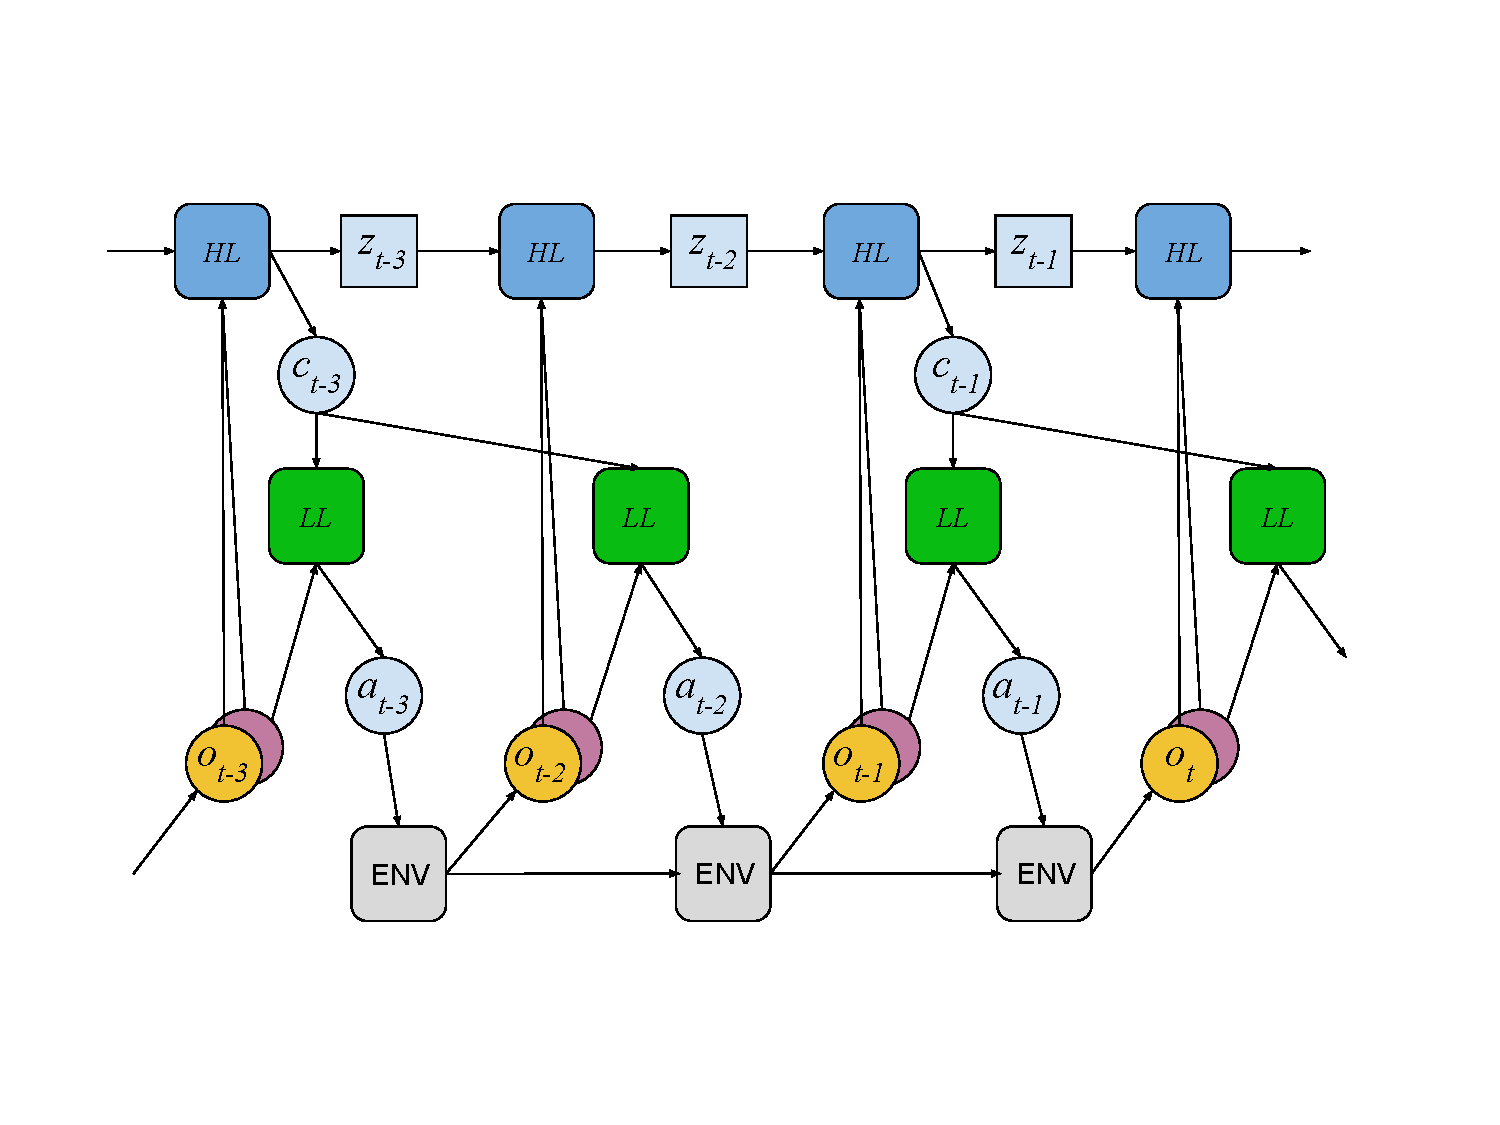
\includegraphics[width=\textwidth]{review_moduler_arch.pdf}
	\centering
	\caption{The hierarchical structure of the modulated controller~\cite{heess2016learning}, which consists
		of the recurrent high-level controller (HL, dark blue) and
		feedforward low-level controller (LL, green).  The
		high-level controller has access to all observations (yellow and red). While both controllers observe sensory
		input at the world-clock frequency, the modulatory con-
		trol signal from the high-level is updated every K
		steps (here K = 2)}
\end{figure}\label{review_moduler_arch}
The hierarchical agent is characterized by a policy $\pi$ with parameter $\theta$. The policy is defined by the composition of the high-level controller $F_H$ and low-level controller $F_L$. The low-level controller is a feed-forward neural network that maps the preprocessed curre
nt state $o(s)$ and the control signal from the high-level controller $c$ to the policy output.
\begin{align}
\pi (a| s) = F_L(o(s),c)
\end{align}
where the preprocessed state $o(s)$ removes task-specific information from the current state.
The high-level controller is a recurrent neural network: $F_H = (f_z,f_c)$ that produces the new control signal at every $K$ time step:
\begin{align}
z_t = f_z(s_t,z_{t-1}) \\
c_t = f_c(z_{t_r})
\end{align}
where $t_r$ is the most recent update output of the control signal. A predefined Gaussian noise component is added to the output $c_t$ during the training of the high level controller, so that the agent has a better performance in exploration.
The training of the hierarchical agent consists of two separate phases: pre-training and transfer. The tasks used for pre-training are relatively simple tasks that facilitate the development of generic locomotion skills. After pre-training, the high-level controller is re-initialized and the weights of low-level controller are frozen. The high-level controller is then trained in the transfer task, which has a sparse reward function.
This method achieves better performance than flat agents on a few realistic robot control tasks. The limitation is that the architecture is highly engineered and domain-specifc. The observation of the low-level agent $o(s)$ need to be designed specifically for each task, and the However, the hierarchical relationships between the two agent, including the pre-training task definition and modulation model, need to be manually predefined. Apart from that, the design of the output modulated signal the high-level agent is limited to several locomotion tasks. This involves the agent. The parameter $K$ is also predefined, and thus the time scale of the high level agent lacks the flexibility.

\subsection{Learning a hierarchical model by meta-learning}
Another work~\cite{frans2017meta}, namely meta learning shared hierarchies (MLSH), proposes a metalearning approach for learning hierarchically structured policies.
The MLSH method formulates the problem as learning a finite set of MDPs $P_M$ with the same state-action space, with a universal agent architecture. The agent consists of two sets of parameters $(\phi,\theta)$, where $\phi$ is the set of task-independent parameters and $\theta$ is the set of task-specific parameters. The meta-learning objective is to optimize the expected return during the agent's entire lifetime:
\begin{align}
\mathrm{maximize}_\phi \mathbb{E}_{M\sim P_M}[R]
\end{align}
The detailed structure of the agent is shown in Figure~\ref{review_mlsh_arch}. The architecture is basically a two-level hierarchical reinforcement learning agent, the components $\phi_1,\phi_2,\dots$ are the parameters of the low-level agent policies (called sub-policies) shared across different tasks and $\theta$ is the parameters of the high-level agent of the current task. The master policy samples the master action at a fixed frequency which selects the acting sub-policies.
\begin{figure}[h]
	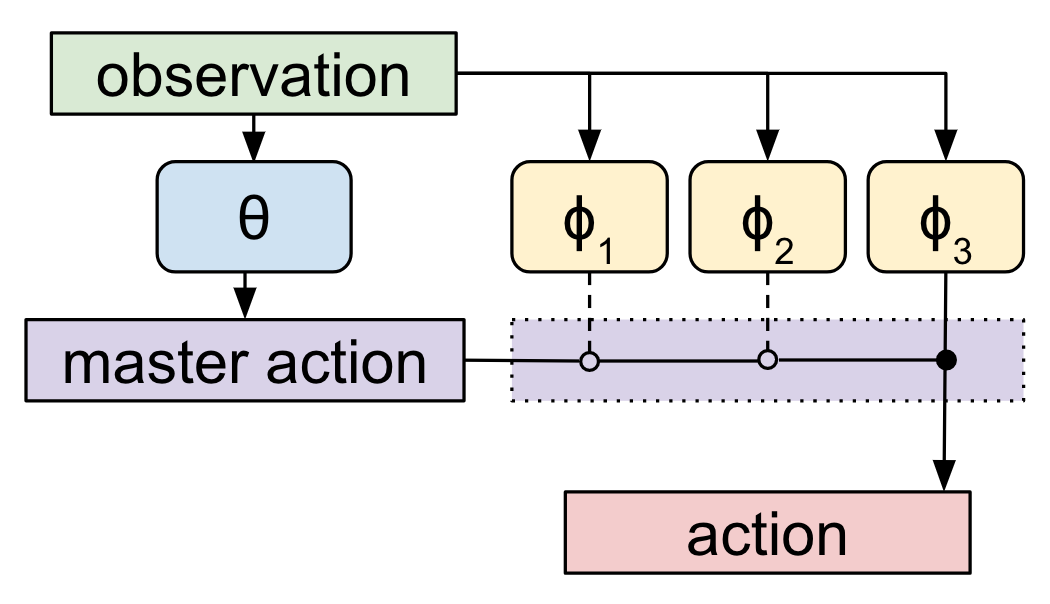
\includegraphics[width=0.5\textwidth]{review_mlsh_setup.png}
	\centering
	\caption{The agent setup of the modulated controller~\cite{frans2017meta},$\theta$ represents the master policy, which selects
		a sub-policy to be active. In the diagram, $\phi_3$ is the active sub-policy, and actions are taken according
		to its output.}
\end{figure}\label{review_mlsh_arch}
The agent is trained in the following manner: First a task is sampled $M$ is sampled and the parameter $\theta$ is re-initialized randomly. Then there is a warmup phase, where only $\theta$ is trained to achieve optimal. Then the agent enters the joint update phase, where both $\theta$ and $\phi$ are updated simutaneously.
The method achieves good performance in several control environments. Including a moving-bandit Ant-robot task, a Ant-robot maze navigation task and an obstacle course task. However the tasks are actually simplified version of the control tasks in \cite{duan2016benchmarking}, where the state of the Ant-robot is periodically reset to prevent episode termination due to the falling over of Ant. That largely reduces the difficulty on learning the locomotion skills of agents. It is not clear whether the method will perform well on the original version of the Ant-robot environment.
The major limitation is that the method relies on a warm up period to learn a high-level agent's policy. However, the authors didn't provide a method to learn the high-level agent's policy $\theta$ at first task, where the parameters $\phi$ are also randomly initialized.
The method also predefines the temporal relationship between the high level policy and low level policy.
% \section{Hindsight Experience Replay}
% The work of~\cite{andrychowicz2017hindsight} generate actuator policies and there corresponding termination predicate policies based on the definition of subgoals. The subgoals are generated by heuristic functions of a target state. TODO
% \section{Scheduled Auxiliary Control}
% The work of \cite{riedmiller2018learning} proposes the method of scheduled auxiliary control. The method generates partial policy by a given set of simple auxiliary tasks, whose reward signals are generated based on heuristic functions of the sensor activation. The method also assume a constant execution length of the actuator policies. TODO
\subsection{Goal-directed learning method}
Several works~\cite{riedmiller2018learning}, ~\cite{andrychowicz2017hindsight} have tried to solve sparse-reward robot control environments through the learning and scheduling of auxiliary policies.
The method of ~\cite{riedmiller2018learning}, namely Scheduled Auxiliary Control (SAC-X), is based on several main principles. First, the original MDP is modified that every state-action pair has a vector rewards, consisting the reward for the original MDP and a set of internal auxiliary rewards. Second, each internal auxiliary reward function is assigned a low-level agent policy, namely intention in this context. Third, there is a high-level scheduler agent that selects and executes the intentions. Fourth, the learning of intentions is performed off-policy on the same experience.
The definitions of internal auxiliary rewards are based on predefined goal states. The  internal auxiliary reward with goal state $g$ is defined as:
\begin{equation}
r_g(s,a)=
\begin{cases}
\delta_g(s),& \text{if } d(s,g)\\
0,              & \text{else}
\end{cases}
\end{equation}
The parameter $\theta$ of the intentions is trained with the aggregation of loss of all the reward functions:
\begin{align}
\mathcal{L}(\theta)  = \mathcal{L}(\theta;M) +\sum_{k=1}^{|A|} (\mathcal{\theta;A_K})
\end{align}
Where $M$ is the MDP with the original reward function and $A=\{A_1,\dots,A_k\}$ is the set of MDPs with internal auxiliary rewards. The training of the intention parameter is formulated as a multi-task RL problem.
The high-level scheduler policy is the trained using an off-policy policy gradient method with $\theta$ being fixed.
The method manages to solve the object grasping and stacking problems in an robot-arm environment. The major limitations of SAC-X is that the method relies on predefined auxiliary MDPs, which is infeasible to obtain in realistic environments.


\subsection{Other methods targeting at sparse environments}
Apart from the above mentioned works, several other methods have also been proposed to solve environments with sparse reward recently, including Unicorn~\cite{mankowitz2018unicorn}, FuN~\cite{vezhnevets2017feudal},  HRL with Stochastic Temporal Grammar~\cite{shu2017hierarchical}, policy sketch method~\cite{andreas2016modular} and strategic attentive writer~\cite{vezhnevets2016strategic}. These methods have only been verified in discrete environments that have relatively low complexity, and involve domain-specific engineering components.